\documentclass[ignorenonframetext,xcolor=x11names]{beamer}

\input{../common.preamble.beamer.tex}
 
\title{Business 4720 - Class 3}

\subtitle{Relational Data}

\begin{document}

\begin{frame}{}
  \titlepage
  \footnotesize
  \input{../license.tex}
\end{frame}

\section{Introduction}

\begin{frame}{This Class}

\begin{block}{What You Will Learn:}
\begin{itemize}
  \item The relational data model
  \item Creating tables and constraints
  \item Querying data for descriptive analytics with SQL
\end{itemize}
\end{block}
\end{frame}

\section{The Relational Data Model}

\begin{frame}{The Relational Data Model}

\begin{block}{Basics}
\begin{itemize}
	\item Tables have columns/fields
	\item Fields are of a primitive data type
\end{itemize}
\end{block}
\begin{block}{Columns Constraints}
\begin{itemize}
	\item \textbf{NOT NULL}: Field must not be empty
	\item \textbf{UNIQUE}: All values in columns must be different
\end{itemize}
\end{block}
\begin{block}{Table Constraints}
\begin{itemize}
	\item \textbf{CHECK}: All values satisfy certain conditions
	\item \textbf{PRIMARY KEY}: Set of fields must uniquely identify a row
	\item \textbf{FOREIGN KEY}: Set of fields whose values must exist in the primary key of another table
\end{itemize}
\end{block}
\end{frame}

\begin{frame}{Foreign Key Constraints}
\begin{itemize}
	\item Express relationships between tables
	\item May reference the same table (''\emph{unary relationship}'') or another table (''\emph{binary relationship}'')
	\item Represent ''1:1'', ''1:Many'', or ''Many:Many'' relationships (''\emph{cardinality}'')
	\item Together with NOT NULL contraints, can represent \emph{optional} relationships
\end{itemize}
\end{frame}

\begin{frame}{Basic SQL Commands}
\renewcommand{\arraystretch}{1.5}

\begin{tabularx}{\textwidth}{l|X} \hline
CREATE TABLE & Creates a new table with specified columns and constraints \\
DROP TABLE & Deletes a table and all its contents \\
INSERT & Inserts a row of data values into a table \\
UPDATE & Updates/modifies data values in a table \\ 
SELECT & Retrieves data values from one or more tables \\ \hline
\end{tabularx}
\end{frame}

\begin{frame}{Basic SQL Commands}
\begin{block}{More Information}
  \begin{itemize}
    \item This course covers only basic information
    \item Further information in PostgreSQL documentation
  \end{itemize}
\end{block}
\vspace{3mm}
\renewcommand{\arraystretch}{1.5}
\small
\begin{tabularx}{\textwidth}{l|X} \hline
  Data Definition & \url{https://www.postgresql.org/docs/current/ddl.html} \\
  Data Types & \url{https://www.postgresql.org/docs/current/datatype.html} \\
  Data Manipulation & \url{https://www.postgresql.org/docs/current/dml.html} \\
  Data Queries & \url{https://www.postgresql.org/docs/current/queries.html} \\
  Functions & \url{https://www.postgresql.org/docs/current/functions.html} \\ \hline
\end{tabularx}
\end{frame}

\begin{frame}{Let's Play with SQL}
\begin{columns}
\begin{column}{.15\textwidth}
\centering 
\includegraphics[width=.8\columnwidth]{postgresql-logo.png}
\end{column}
\begin{column}{.85\textwidth}
\begin{itemize}
  \item PostgreSQL RDBMS installed in the course virtual machine
  \item Access options
  \begin{enumerate}
     \item psql command line access
     \item DBeaver graphical user interface
     \item pgAdmin administration application
  \end{enumerate}
\end{itemize}
\end{column}
\end{columns}
\end{frame}

\begin{frame}{PostgreSQL Database Management System}
\begin{itemize}
  \item A DBMS is a background program without user interface
  \item Runs on one computer (''server'') or distributed across a cluster of multiple computers
  \begin{itemize}
    \item \emph{The name of the local computer is called ''localhost''}
  \end{itemize}
  \item Administration tools allow basic manual interaction
  \begin{itemize}
    \item pgAdmin offers easy tools for creating tables and querying data, but we will use the SQL language instead
  \end{itemize}
  \item A DBMS can manage multiple databases
  \begin{itemize}
    \item \emph{Your database is called ''busi4720''}
  \end{itemize}
  \item A database may have multiple schema
  \begin{itemize}
    \item A schema is a grouping of tables and related info
    \item \emph{The default schema is called ''public''}
  \end{itemize}
  \item A schema may contain multiple tables (and related information)
\end{itemize}
\end{frame}


\begin{frame}{PSQL}
\begin{itemize}
   \item Type \texttt{psql} in a terminal window
   \item The psql command \texttt{\textbackslash conninfo} shows connection info
   \item Quit psql using \texttt{\textbackslash q}
   \item You should be connected to the ''busi4720'' database
   \item \textbf{Tip}: Use a notepad application to assemble your SQL commands to paste into psql
\end{itemize}
\centering
\includegraphics[width=\textwidth]{screen3.png}
\end{frame}

\begin{frame}{DBeaver}
\begin{itemize}
   \item Navigate to and select the ''busi4720'' database in the navigator on the left
   \item In the toolbar, press the ''SQL'' button
\end{itemize}
\vspace{3mm}
\centering
\includegraphics[width=.8\textwidth]{screen4.png}
\end{frame}

\begin{frame}[fragile]{PostgreSQL Hands-On with pgAdmin}
\begin{itemize}
  \item Navigate to and select the ''busi4720'' database in the object explorer on the left
  \item From the ''Tools'' menu, select the ''Query tool''
\end{itemize}
\vspace{3mm}
\centering
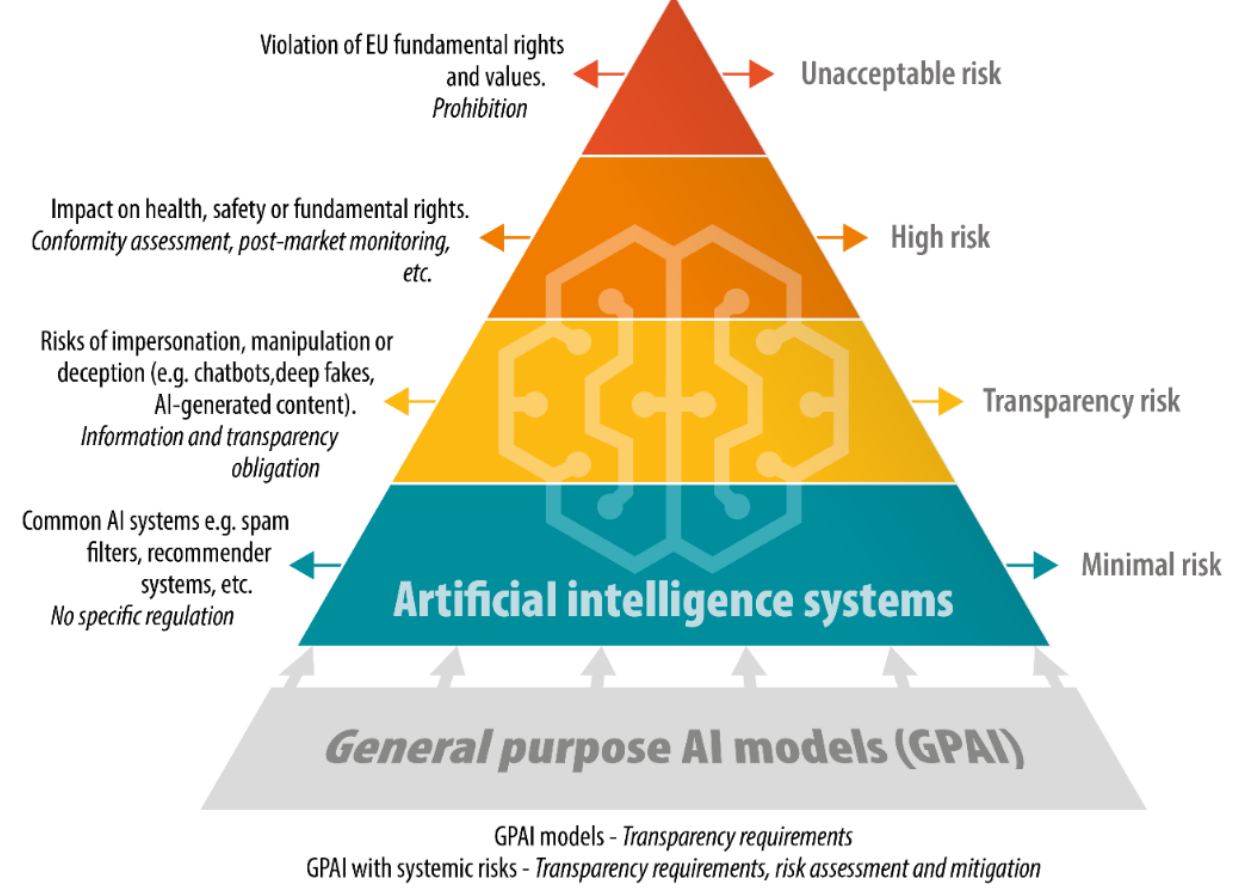
\includegraphics[width=\textwidth]{screen2.png}
\end{frame}

\begin{frame}[fragile]{PostgreSQL Hands-On}
\begin{itemize}
\item Enter the following query:
\begin{itemize}
    \item In psql, just press \colorbox{lightgray}{RETURN} to execute
    \item In DBeaver, press \colorbox{lightgray}{CTRL-RETURN} to execute
    \item In pgadmin, press \colorbox{lightgray}{F5} to execute
\end{itemize}
\end{itemize}
\footnotesize
\begin{sqlcode}
CREATE TABLE products (
  pcode integer,
  name  varchar(100),
  price float4,
  PRIMARY KEY (pcode) );
\end{sqlcode}
\normalsize
\vspace{-5mm}
\begin{block}{Tips}
\begin{itemize}
  \item All SQL commands must end with a semicolon
  \item Capitilization does not matter
\end{itemize}
\end{block}
\end{frame}

\begin{frame}[fragile]{PostgreSQL Hands-On}
\begin{itemize}
  \item Create a table for the suppliers as well:
\end{itemize}
\footnotesize
\begin{sqlcode}
CREATE TABLE suppliers (
  scode integer,
  name  varchar(100),
  city  varchar(100),
  PRIMARY KEY (scode) );
\end{sqlcode}
\normalsize
\begin{itemize}
  \item Insert some data into the tables:
\end{itemize}
\footnotesize
\begin{sqlcode}
INSERT INTO products VALUES (1, 'Hex Bolt', 1.99);
INSERT INTO products VALUES (2, 'Round Bolt', 2.99);

INSERT INTO suppliers VALUES (1, 'Bolts Inc', 'HVGB');
INSERT INTO suppliers 
    VALUES (2, 'Hardware Co', 'Cartwright');
\end{sqlcode}
\vspace{5mm}
\end{frame}

\begin{frame}[fragile]{PostgreSQL Hands-On}
\begin{itemize}
  \item Check that the data is there:
\end{itemize}
\footnotesize
\begin{sqlcode}
SELECT * FROM products;
SELECT * FROM suppliers;
\end{sqlcode}
\normalsize
\begin{itemize}
  \item Can we capture which supplier supplies which product?
  \item We need a foreign key!
  \item Let's delete our ''products'' table and rework it
\end{itemize}
\footnotesize
\begin{sqlcode}
DROP TABLE products;
\end{sqlcode}

\end{frame}

\begin{frame}[fragile]{PostgreSQL Hands-On}
\begin{itemize}
  \item \textbf{Assumption}: Suppliers supply many products, a product may be supplied by only one supplier
\end{itemize}
\footnotesize
\begin{sqlcode}
CREATE TABLE products (
  pcode    integer,
  name     varchar(100),
  price    float4,
  supplier integer,
  PRIMARY KEY (pcode),
  FOREIGN KEY (supplier) REFERENCES suppliers );
\end{sqlcode}
\end{frame}

\begin{frame}[fragile]{PostgreSQL Hands-On}
\begin{itemize}
  \item Insert some product data:
\end{itemize}
\footnotesize
\begin{sqlcode}
INSERT INTO products VALUES(1, 'Hex Bolt', 1.99, 1);
INSERT INTO products VALUES(2, 'Round Bolt', 2.99, 1);
INSERT INTO products 
    VALUES(3, 'Square Bolt', 3.99, NULL);
\end{sqlcode}
\normalsize
\begin{itemize}
  \item There are products that have no supplier (the ''square bolt'')
  \item There are suppliers that supply many products (supplier 1)
  \item There are suppliers that do not supply products (supplier 2)
  \item \emph{We cannot record multiple suppliers for each product!}
\end{itemize}
\end{frame}

\begin{frame}[fragile]{PostgreSQL Hands-On}
\begin{itemize}
  \item Make sure that every product has a supplier:
\end{itemize}
\footnotesize
\begin{sqlcode}
DROP TABLE IF EXISTS products;

CREATE TABLE products (
  pcode    integer,
  name     varchar(100),
  price    float4,
  supplier integer NOT NULL,
  PRIMARY KEY (pcode),
  FOREIGN KEY (supplier) REFERENCES suppliers );
\end{sqlcode}
\end{frame}

\begin{frame}[fragile]{PostgreSQL Hands-On}
\begin{itemize}
  \item Can products be supplied by multiple suppliers?
  \item We need another table, representing the ''supplies'' relationship, a ''Many:Many'' relationship
  \item Let's drop everything and start again!
\end{itemize}
\footnotesize
\begin{sqlcode}
DROP TABLE IF EXISTS products;
DROP TABLE IF EXISTS suppliers;
\end{sqlcode}
\normalsize
  \begin{itemize}
    \item \emph{Tip}: Must drop tables in correct order because of foreign keys!
  \end{itemize}
\end{frame}

\begin{frame}[fragile]{PostgreSQL Hand-On}
\footnotesize
\begin{sqlcode}
CREATE TABLE products (
  pcode integer,
  name  varchar(100),
  PRIMARY KEY (pcode) );
  
CREATE TABLE suppliers (
  scode integer,
  name  varchar(100),
  city  varchar(100),
  PRIMARY KEY (scode) );
  
CREATE TABLE supplies (
  scode  integer NOT NULL,
  pcode  integer NOT NULL,
  price  float4 NOT NULL,
  PRIMARY KEY (scode, pcode),
  FOREIGN KEY (scode) REFERENCES suppliers,
  FOREIGN KEY (pcode) REFERENCES products );
\end{sqlcode}
\end{frame}

\begin{frame}[fragile]{PostgreSQL Hand-On}
\footnotesize
\begin{sqlcode}
INSERT INTO products VALUES (1, 'Hex Bolt');
INSERT INTO products VALUES (2, 'Round Bolt');

INSERT INTO suppliers VALUES (1, 'Bolts Inc', 'HVGB');
INSERT INTO suppliers 
    VALUES (2, 'Hardware Co', 'Cartwright');

INSERT INTO supplies VALUES(1, 1, 1.99);
INSERT INTO supplies VALUES(1, 2, 2.49);
INSERT INTO supplies VALUES(2, 1, 2.99);
INSERT INTO supplies VALUES(2, 2, 1.79);
\end{sqlcode}
\end{frame}

\begin{frame}{Foreign Key Summary}
\small
\begin{block}{1:Many Relationship}
\begin{itemize}
  \item Requires a foreign key from the ''many'' table into the ''one'' table
  \item \textbf{Example}: A supplier supplies many products but a product has one supplier (or none, depending on NOT NULL constraint)
\end{itemize}
\end{block}
\begin{block}{Many:Many Relationship}
\begin{itemize}
  \item Requires a table that represents the relationship
  \item Foreign keys from this table reference the ''main'' tables
  \item \textbf{Example}: A supplier supplies many products and a product can be supplied by many suppliers
  \item Can be extended to relationships between three or more tables
  \item \textbf{Example}: A supplier supplies many products from multiple warehouses
\end{itemize}
\end{block}
\end{frame}

\begin{frame}{Hands-On Exercise}
\small
\begin{enumerate}
  \item Consider the following:
	\begin{itemize}
	  \item A book has an ISBN number and a title. 
	  \item An author has a name and an address. 
	  \item An author can write many books, and a book can be written by multiple authors. A book is written in a certain year.
	\end{itemize}
  \item Write the CREATE TABLE statements with the necessary FOREIGN KEY statements, and execute them on PostgreSQL
  \begin{itemize}
    \item Use appropriate datatypes for the columns
    \item Create an appropriate PRIMARY KEY for all tables
  \end{itemize}
  \item Use INSERT statements to create some example data
  \item Use SELECT statements to ensure your data exists
\end{enumerate}
\end{frame}

\begin{frame}{Querying Data with SQL}
\begin{block}{Parts of the SELECT statement}
  \begin{itemize}
     \item \textbf{SELECT}: which columns to query
     \item \textbf{FROM}: which tables to query from
     \item \textbf{JOIN}: how to combine data from multiple tables
     \item \textbf{WHERE}: conditions on field values
     \item \textbf{GROUP BY}: groups within which to aggregate data
     \item \textbf{HAVING}: conditions on group aggregate values
     \item \textbf{ORDER BY}: how to sort the result
     \item \textbf{LIMIT}: how many results to return
   \end{itemize}
\end{block}
\end{frame}

\begin{frame}[fragile]{Querying -- Simple Example}
Set up tables with 1:Many relationship:
\footnotesize
\begin{sqlcode}
DROP TABLE IF EXISTS products;
DROP TABLE IF EXISTS suppliers;

CREATE TABLE suppliers (
scode integer,
name varchar(100),
city varchar(100),
PRIMARY KEY (scode) );

CREATE TABLE products (
pcode	integer,
name	varchar(100),
price	float4,
scode   integer,
PRIMARY KEY (pcode),
FOREIGN KEY (scode) REFERENCES suppliers );
\end{sqlcode}
\end{frame}

\begin{frame}[fragile]{Querying -- Simple Example}
Insert some data:
\footnotesize
\begin{sqlcode}
INSERT INTO SUPPLIERS VALUES (1, 'Bolts Inc', 'HVGB');
INSERT INTO SUPPLIERS VALUES (2, 'Hardware Co', 'Cartwright');

INSERT INTO products VALUES(1, 'Hex Bolt A', 1.99, 1);
INSERT INTO products VALUES(2, 'Round Bolt 1', 2.99, 1);
INSERT INTO products VALUES(3, 'Square Bolt B', 3.99, 1);
INSERT INTO products VALUES(4, 'Hex Bolt B', 2.99, 1);
INSERT INTO products VALUES(5, 'Round Bolt 2', 1.99, 2);
INSERT INTO products VALUES(6, 'Square Bolt 7', 3.49, 2);
\end{sqlcode}
\end{frame}

\begin{frame}[fragile]{Querying -- Simple Example}
Select all columns from products table:
\begin{sqlcode}
SELECT * FROM products;
\end{sqlcode}
Select all columns from products table for supplier 1:
\begin{sqlcode}
SELECT * FROM products WHERE scode = 1;
\end{sqlcode}
Select some columns from products table with price < 3:
\begin{sqlcode}
SELECT name, supplier FROM products WHERE price < 3;
\end{sqlcode}
Select all columns from products, ordered by ascending price and then descending name:
\begin{sqlcode}
SELECT * FROM products ORDER BY price ASC, name DESC;
\end{sqlcode}
Select the names of the 3 cheapest products:
\begin{sqlcode}
SELECT name FROM products ORDER BY price ASC LIMIT 3;
\end{sqlcode}
\end{frame}

\begin{frame}[fragile]{Querying -- Join Tables}
Select products and the names of their suppliers:
\begin{sqlcode}
SELECT * FROM products INNER JOIN suppliers USING (scode);

-- (Almost) Equivalent:
SELECT * FROM products 
    INNER JOIN suppliers ON products.scode=suppliers.scode;

SELECT * FROM products, suppliers 
    WHERE products.scode=suppliers.scode;
\end{sqlcode}
Rename columns for clarity:
\begin{sqlcode}
SELECT products.name AS "Product", 
       price AS "Price", 
       suppliers.name AS "Supplier", 
       city AS "Location"
    FROM products INNER JOIN suppliers USING (scode);
\end{sqlcode}
\end{frame}

\begin{frame}{Types of Joins}
\renewcommand{\arraystretch}{1.5}
Types of joins between tables T1 and T2: \\

\small
\begin{tabularx}{\textwidth}{l|X} \hline
INNER & Selects only rows from T1 that have corresponding row in T2 and vice versa. \\
LEFT OUTER & Selects all rows from T1, if T2 does not have a corresponding row, NULL values are inserted. \\
RIGHT OUTER & Select all rows from T2, if T1 does not have a corresponding row, NULL values are inserted. \\
FULL OUTER & Selects all rows from T1, T2. If the other table is missing corresponding row, NULL values are inserted. \\ \hline
\end{tabularx}
\end{frame}


\begin{frame}[fragile]{Querying -- Groups and Aggregates}
Select the number of products for each supplier:
\begin{sqlcode}
SELECT scode, count(*) from products GROUP BY scode;
\end{sqlcode}
Add the name of suppliers by joining suppliers table:
\begin{sqlcode}
SELECT suppliers.name, count(*)
    FROM suppliers INNER JOIN products USING (scode)
    GROUP BY scode;
\end{sqlcode}
Mean price of products for each supplier, ordered descending:
\begin{sqlcode}
SELECT suppliers.name, AVG(price)
    FROM suppliers INNER JOIN products USING (scode)
    GROUP BY scode
    ORDER BY AVG(price) DESC;
\end{sqlcode}
Find only suppliers for which average price less than 2.80:
\begin{sqlcode}
SELECT suppliers.name, AVG(price)
    FROM suppliers INNER JOIN products USING (scode)
    GROUP BY scode
    HAVING AVG(price) < 2.8;
\end{sqlcode}
\end{frame}

\begin{frame}{Frequently Used Aggregation Functions}
\renewcommand{\arraystretch}{1.5}
Standard SQL: \\

\small
\begin{tabular}{l|l|l|l|l} \hline
MIN() & MAX() & COUNT() & SUM() & AVG() \\ \hline
\end{tabular}
\normalsize

\vspace{\baselineskip}
PostgreSQL (excerpt):\\

\small
\begin{tabular}{l|l|l} \hline
CORR() & STDDEV() & VARIANCE() \\
MODE() & PERCENTILE() & REGR\_SLOPE() \\
REGR\_R2() & RANK() & DENSE\_RANK() \\ \hline
\end{tabular}

\end{frame}


\begin{frame}{Relational Diagrams}
\begin{itemize}
  \item Graphically show the relationships in a database model
  \item Often called ''\emph{Entity-Relationship diagram}'' (but that is not quite correct)
  \item Useful for understanding the structure of the data
  \item Useful for writing queries with many JOINs
  \item Can be automatically created from an existing database
  \begin{itemize}
     \item In the \textbf{pgAdmin} Object Explorer, right-click on the ''busi4720'' database, select ''ERD for Database''
     \item In the \textbf{DBeaver} Navigator, select the ''busi4720'', then the ''public'' schema, then right click and select ''View Diagram''
  \end{itemize}
\end{itemize}
\end{frame}

\begin{frame}{Relational Diagram for the Pagila Database}
\centering
\includegraphics[height=3in]{pagila2dbeaver.png}
\end{frame}

\begin{frame}{The Pagila Demo Database}

\begin{itemize}
  \item Based on the Sakila database\footnote{\scriptsize\url{https://dev.mysql.com/doc/sakila/en/}, 
\url{https://dev.mysql.com/doc/sakila/en/sakila-license.html}}, ported to PostgreSQL\footnote{\scriptsize\url{https://github.com/devrimgunduz/pagila},
\url{https://github.com/devrimgunduz/pagila/blob/master/LICENSE.txt}}
  \item Pre-installed in the course virtual machine
  \item DVD rental case with main tables:
  \begin{itemize}
	\item \textbf{Film}: has many categories, is in inventory at many stores
	\item \textbf{Store}: has many films in inventory, has a staff manager
	\item \textbf{Customer}: may have many rentals, associated with a store
	\item \textbf{Actor}: may appear in many films, films have many actors
	\item \textbf{Inventory}: stores have many films in inventory, and film may be in inventory in many stores
	\item \textbf{Rental}: Inventory is rented by customer through staff
	\item \textbf{Staff}: Staff are associated with a store
	\item \textbf{Address}: Stores, customers, and staff have an addresses
  \end{itemize}
\end{itemize}
\end{frame}

\begin{frame}[fragile]{Querying Data with SQL}
Find all actors and the films they appeared in, ordered by film category and year, for those films that are rated PG:
\footnotesize
\begin{sqlcode}
SELECT concat(left(actor.first_name, 1), 
              '. ', actor.last_name) AS Actor, 
       category.name AS Category, 
       film.title, 
       film.release_year
  FROM film_actor
  INNER JOIN actor USING (actor_id)
  INNER JOIN film USING (film_id)
  INNER JOIN film_category USING (film_id)
  INNER JOIN category USING (category_id)
  WHERE film.rating = 'PG'
  ORDER BY actor.last_name, 
           actor.first_name, 
           category.name ASC, 
           film.release_year DESC, 
           film.title ASC;
\end{sqlcode}
\end{frame}

\begin{frame}[fragile]{Querying Data with SQL}
Equivalent alternative without using JOIN:
\footnotesize
\begin{sqlcode}
SELECT concat(left(actor.first_name, 1), 
              '. ', actor.last_name) AS Actor, 
       category.name AS Category, 
       film.title, 
       film.release_year
  FROM film_actor, film, actor, film_category, category
  WHERE actor.actor_id = film_actor.actor_id AND
        film.film_id = film_actor.film_id AND
        film_category.film_id = film.film_id AND
        category.category_id = film_category.category_id AND
        film.rating = 'PG'
  ORDER BY actor.last_name, 
           actor.first_name, 
           category.name ASC, 
           film.release_year DESC, 
           film.title ASC;
\end{sqlcode}
\end{frame}

\begin{frame}[fragile]{Querying Data with SQL}
Find the most popular actors in the rentals in each city:
\footnotesize
\begin{sqlcode}
SELECT city.city, 
       concat(actor.first_name, '. ', 
           actor.last_name) AS actor_name,
       count(concat(actor.first_name, '. ', 
           actor.last_name)) AS Number_Rentals
  FROM rental
  INNER JOIN inventory USING (inventory_id)
  INNER JOIN store USING (store_id)
  INNER JOIN address USING (address_id)
  INNER JOIN city USING (city_id)
  INNER JOIN film USING (film_id)
  INNER JOIN film_actor USING (film_id)
  INNER JOIN actor USING (actor_id)
  GROUP BY city.city, actor.actor_id
  HAVING count(rental.rental_id) >= 300
  ORDER BY city ASC, 
           Number_Rentals DESC, 
           actor_name ASC;
\end{sqlcode}
\end{frame}

\begin{frame}[fragile]{Querying Data with SQL}
Find the customers who spent the most, with their phone numbers and cities, the cities their store is in, and the number of rentals with the highest total rental payments for each category grouped by city of the rental store:
\scriptsize
\begin{sqlcode}
SELECT category.name AS category_name, 
       store_city.city AS store_city,
       customer.customer_id, 
       concat(customer.first_name, ' ', 
          customer.last_name) AS customer_name,
       cust_city.city AS customer_city,
       cust_address.phone AS customer_phone,
       count(rental.rental_id) AS num_rentals,
       sum(amount) AS total_amount
 FROM city AS cust_city, city AS store_city, 
      address AS cust_address, address AS store_address, 
      store, rental
 INNER JOIN payment USING (customer_id)
 INNER JOIN customer USING (customer_id)
 INNER JOIN inventory USING (inventory_id)
 INNER JOIN film USING (film_id)
 INNER JOIN film_category USING (film_id)
 INNER JOIN category USING (category_id)
\end{sqlcode}
\end{frame}
\begin{frame}[fragile]{Cont'd}
\scriptsize
\begin{sqlcode}
 WHERE store.store_id = inventory.store_id
   AND store_address.address_id = store.address_id
   AND store_city.city_id = store_address.city_id
   AND cust_address.address_id = customer.address_id
   AND cust_city.city_id = cust_address.city_id
 GROUP BY category.name, customer.customer_id, 
         cust_address.address_id, cust_city.city, 
         store_city.city
 HAVING sum(amount) IN (
  SELECT sum(amount) AS maxamount
   FROM store, address, city AS inner_city, rental
   INNER JOIN payment USING (customer_id)
   INNER JOIN customer USING (customer_id)
   INNER JOIN inventory USING (inventory_id)
   INNER JOIN film USING (film_id)
   INNER JOIN film_category USING (film_id)
   INNER JOIN category AS inner_category USING (category_id)
\end{sqlcode}
\end{frame}
\begin{frame}[fragile]{Cont'd}
\scriptsize
\begin{sqlcode}
   WHERE inner_category.name = category.name AND
         inner_city.city = store_city.city AND
         store.store_id = inventory.store_id AND
         address.address_id = store.address_id AND
         inner_city.city_id = address.city_id
   GROUP BY inner_category.name, 
            inner_city.city, 
            customer.customer_id
   ORDER BY inner_category.name ASC, 
            inner_city.city, 
            maxamount DESC
   LIMIT 1 )
 ORDER BY category.name ASC, store_city ASC;
\end{sqlcode}
\end{frame}

\begin{frame}[fragile]{Querying Data with SQL}
Get the total rental revenue and number of rentals for each store by month:
\scriptsize
\begin{sqlcode}
SELECT city.city, 
       extract(year from payment_date) AS year, 
       extract(month from payment_date) AS month, 
       sum(amount) as dollars, 
       count(rental.rental_id) as rentals
FROM payment, rental, inventory, store, address, city
WHERE payment.rental_id = rental.rental_id AND
      rental.inventory_id = inventory.inventory_id AND
      inventory.store_id = store.store_id AND
      store.address_id = address.address_id AND
      address.city_id = city.city_id
GROUP BY city.city, 
         extract(year from payment_date), 
         extract(month from payment_date)
ORDER BY city.city, 
         extract(year from payment_date), 
         extract(month from payment_date);
\end{sqlcode}
\end{frame}

\begin{frame}[fragile]{Querying Data with SQL}
Get the top 5 and the bottom 5 grossing customers by year
\scriptsize
\begin{sqlcode}
( SELECT concat(customer.first_name, ' ', 
             customer.last_name) AS customer_name,
       extract(year from payment_date) AS year, 
       sum(amount) as dollars,
       'Top-5' as note
FROM payment, customer
WHERE payment.customer_id = customer.customer_id
GROUP BY extract(year from payment_date),customer.customer_id
ORDER BY dollars DESC LIMIT 5
) UNION (
SELECT concat(customer.first_name, ' ', 
           customer.last_name) AS customer_name,
       extract(year from payment_date) AS year, 
       sum(amount) as dollars,
       'Bottom-5' as note
FROM payment, customer
WHERE payment.customer_id = customer.customer_id
GROUP BY extract(year from payment_date),customer.customer_id
ORDER BY dollars ASC LIMIT 5 ) 
ORDER BY dollars DESC;
\end{sqlcode}
\end{frame}

\begin{frame}{Tips on Querying Data with SQL}
\begin{itemize}
  \item Subqueries are intuitive but not efficient
  \item Use set operations to combine results from multiple queries (UNION, INTERSECT, EXCEPT)
  \item Use DISTINCT to query unique values
  \item Postgres can import/export from/to CSV and JSON files
\end{itemize}
\end{frame}

\begin{frame}{Hands-On Exercises}
\begin{enumerate}
  \item Find the names and the rental numbers of the top 5 customers who rented the most films
  \begin{itemize}
    \item \textbf{Tip}: Join tables ''rental'', ''customer'', use ''group by'' and the ''count()'' function
  \end{itemize}
  \item Calculate the rental revenue per customer. Who are the top 5? Bottom 5?
  \begin{itemize}
    \item \textbf{Tip}: Join tables ''rental'', ''customer'', ''payment'', use ''group by'' and the ''sum()'' function
  \end{itemize}
  \item Calculate the average rental revenue per customer for each store
  \begin{itemize}
    \item \textbf{Tip}: Join tables ''rental'', ''customer'', ''payment'', ''inventory'', use ''group by'' and the ''avg()'' function
  \end{itemize}
\end{enumerate}
\end{frame}

\begin{frame}{Hands-On Exercises \small [cont'd]}
\begin{enumerate}
  \setcounter{enumi}{3}
  \item Calculate the rental counts for each country of customer. Are there countries with no rentals?
  \begin{itemize}
    \item \textbf{Tip}: Join tables ''rental'', ''customer'', ''address'', ''city'', ''country'', use ''group by'' and the ''count()'' function
  \end{itemize}
  \item Find all films with a single actor
  \begin{itemize}
    \item \textbf{Tip}: Join tables ''film'', ''film\_actor'', use ''group by'' and the ''count()'' function with a HAVING clause
  \end{itemize}
  \item Create tables to represent a part-of hiearchy. For example, a product may be a part of another product, and prodcuts may have multiple parts.
  \begin{itemize}
    \item \textbf{Tip}: You need only one table
  \end{itemize}
\end{enumerate}
\end{frame}


\end{document}
